\documentclass{article}
% translate with >> pdflatex -shell-escape <file>

% This file is used as unit test for pgfplots, copyright by Christian Feuersaenger.
% 
% See
%   http://pgfplots.sourceforge.net/pgfplots.pdf
% for pgfplots.
%
% Any required input files (for <plot table> or <plot file> or the table package) can be downloaded
% at
% http://www.ctan.org/tex-archive/graphics/pgf/contrib/pgfplots/doc/latex/
% and
% http://www.ctan.org/tex-archive/graphics/pgf/contrib/pgfplots/doc/latex/plotdata/

\usepackage{pgfplots}
\pgfplotsset{compat=newest}

\pagestyle{empty}

\begin{document}
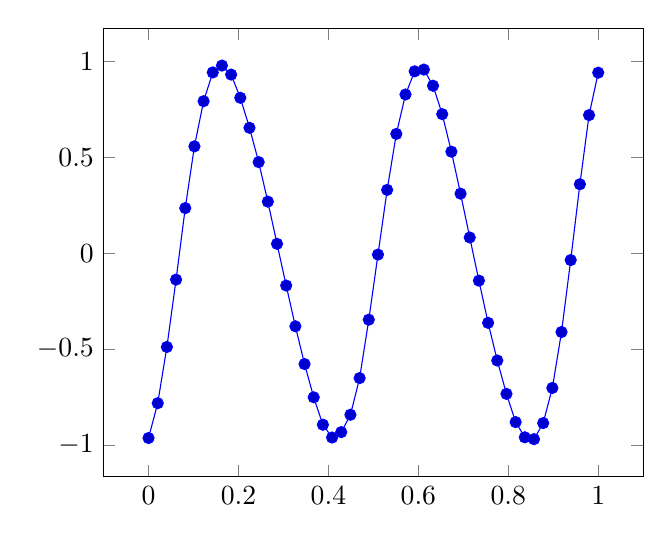
\begin{tikzpicture}%
\begin{axis}
\addplot plot coordinates {
	(0.000000,	-0.963159)
	(0.020408,	-0.781664)
	(0.040816,	-0.488585)
	(0.061224,	-0.137738)
	(0.081633,	0.234861)
	(0.102041,	0.556489)
	(0.122449,	0.791942)
	(0.142857,	0.941856)
	(0.163265,	0.977486)
	(0.183673,	0.930499)
	(0.204082,	0.809581)
	(0.224490,	0.653308)
	(0.244898,	0.474588)
	(0.265306,	0.268631)
	(0.285714,	0.048692)
	(0.306122,	-0.168568)
	(0.326531,	-0.380963)
	(0.346939,	-0.577633)
	(0.367347,	-0.751043)
	(0.387755,	-0.893755)
	(0.408163,	-0.960465)
	(0.428571,	-0.932380)
	(0.448980,	-0.841830)
	(0.469388,	-0.650880)
	(0.489796,	-0.346509)
	(0.510204,	-0.007265)
	(0.530612,	0.329744)
	(0.551020,	0.621489)
	(0.571429,	0.826905)
	(0.591837,	0.947602)
	(0.612245,	0.956706)
	(0.632653,	0.872426)
	(0.653061,	0.724325)
	(0.673469,	0.528915)
	(0.693878,	0.310032)
	(0.714286,	0.081807)
	(0.734694,	-0.143046)
	(0.755102,	-0.363063)
	(0.775510,	-0.559141)
	(0.795918,	-0.733031)
	(0.816327,	-0.880063)
	(0.836735,	-0.959350)
	(0.857143,	-0.968957)
	(0.877551,	-0.885145)
	(0.897959,	-0.702171)
	(0.918367,	-0.410704)
	(0.938776,	-0.035900)
	(0.959184,	0.359062)
	(0.979592,	0.719407)
	(1.000000,	0.940563)
};
\end{axis}
\end{tikzpicture}
\end{document}
